%!TEX root=vissoft.tex

\section{Service Utilization}
\label{sec:util}

  The most fundamental insight that a service maintainer needs regards service utilization. %\vspace{0.5cm}

  Figure \ref{fig:aeu} shows a first perspective on endpoint utilization that \tool provides: a stacked bar chart of the number of hits to various endpoints grouped by day. Figure~\ref{fig:aeu} in particular shows that at its peak the API has about 12.000 hits per day. 
  The way users interact with the platform can also be inferred since the endpoints are indicators of different activity types, e.g.: 

  \begin{enumerate}

    \item \epTranslations is an indicator of the amount of foreign language reading the users are doing, and 

    \item {\color{mygreen} \epOutcome} is an indicator of the amount of foreign vocabulary practice the users are doing.

  \end{enumerate}


  \begin{figure}[!ht]
    \centering
    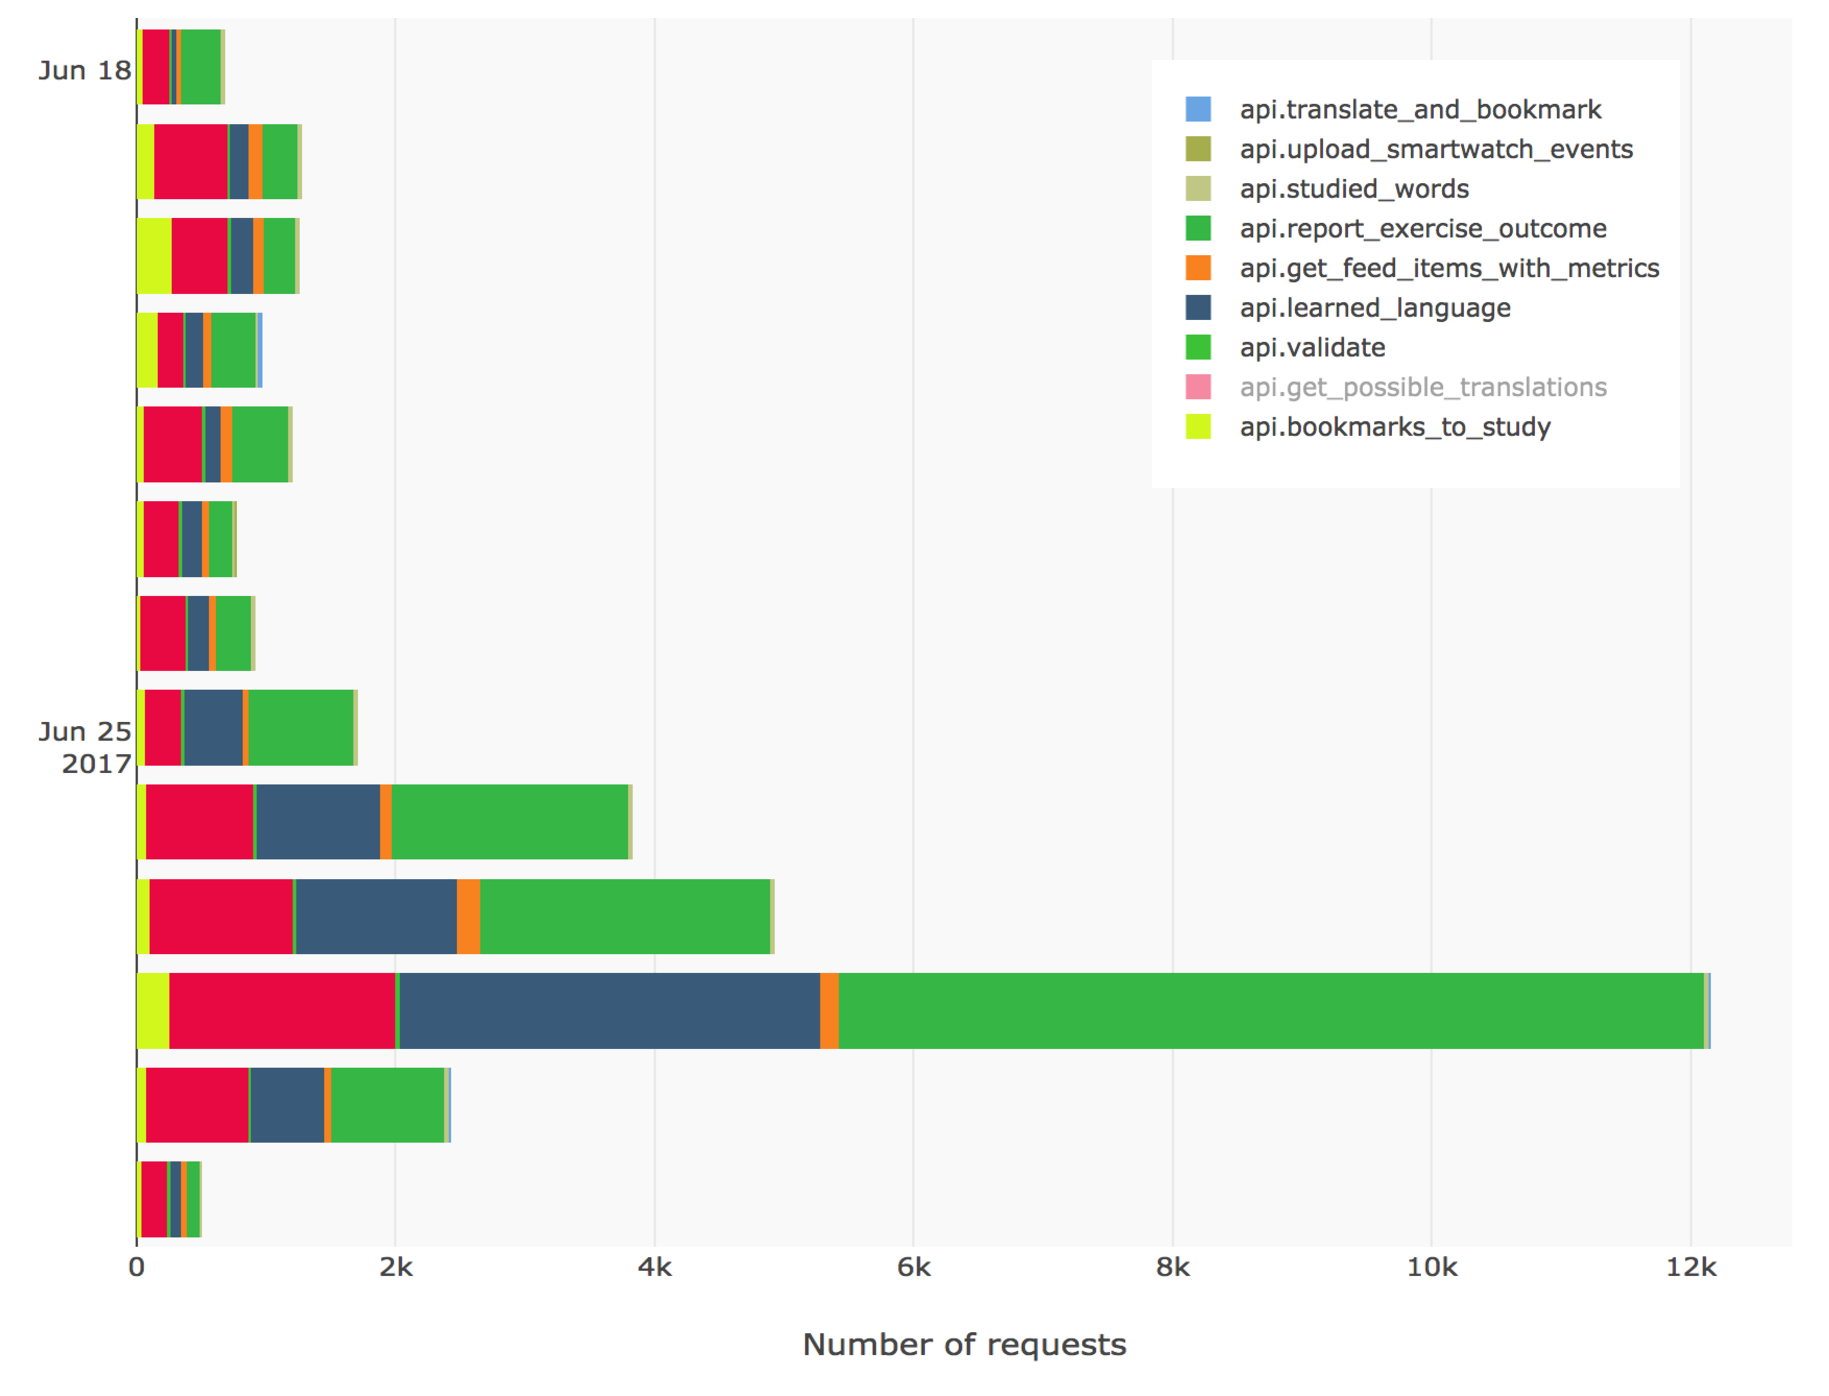
\includegraphics[width=\linewidth]{number_of_requests_}
    \caption{The number of requests per endpoint per day view shows the overall utilization of the monitored application}
    \label{fig:aeu}
  \end{figure}

  Besides showing the overall utilization, this endpoint provides the maintainer with information relevant for decisions regarding endpoint deprecation --- one of the most elementary ways of {\em understanding the needs of the downstream}\cite{Haen14a}. In our case study, the maintainer realized that several endpoints which they thought were not being used, contrary to their expectations, were actually very much in use\footnote{Usage information can also be used to increase the confidence of the maintainer that a given endpoint is not used, although it can never be used a proof.}.

  \niceseparator

%   \todo{Add the time series graph and discuss it before the heatmap? We can then sell the heatmap better} 
%   \ml{Not sure about which graph you refer to here V}

  A second type of utilization question that the \tool can answer automatically regards {\em cyclic patterns of usage per hour of day} by means of a heatmap, as in \Fref{fig:dp}. 

  % \mltp{ can we add vertical lines that highlight the beginning of a new week (e.g. before Sunday): }
  % Patrick: adding separators in the graph is unfortunately not supported by the library.

    \begin{figure}[!ht]
      \centering
      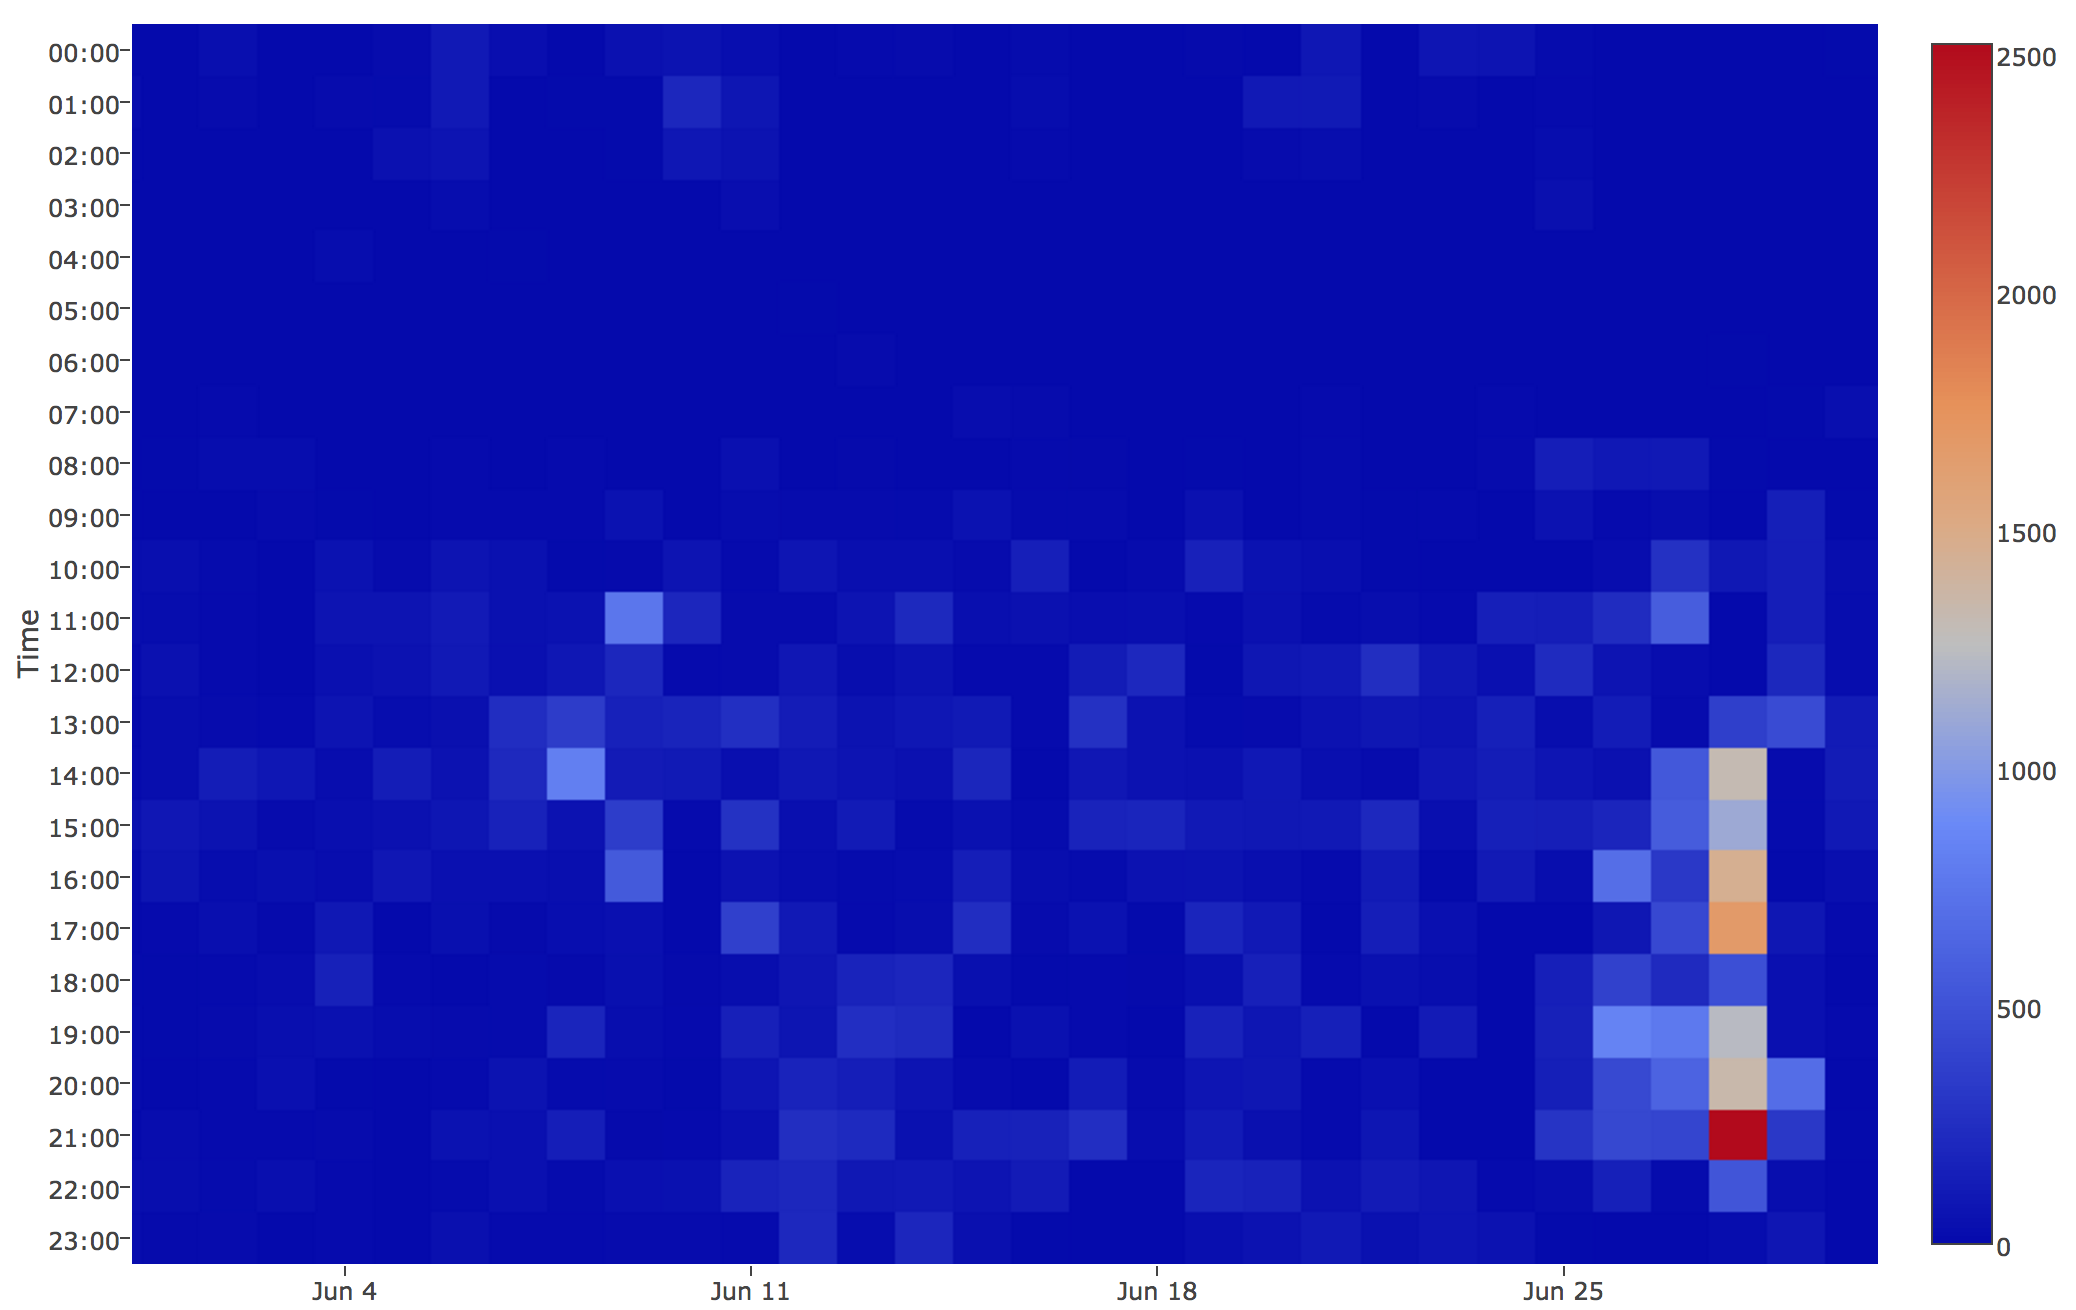
\includegraphics[width=0.8\linewidth]{daily_patterns_}
      \caption{Usage patterns become easy to spot in the requests per hour heatmap}
      \label{fig:dp}
    \end{figure}


  Figure \ref{fig:dp} shows the API not being used during the early morning hours, with most of the activity focused around working hours and some light activity during the evening. This is consistent with the fact that the current users are all in the central European timezone. Also, the figure shows that the spike in utilization that was visible also in the previous graph happended in on afternoon/evening.

